\chapter{Infraestructura}\label{cap.infraestructura}
En este capitulo se describirán las tecnologías sobre las que se cimienta este trabajo. Para empezar, se detallara el funcionamiento del framework Electron, ya que todo el desarrollo de este trabajo sera compatible con él. Se profundizara en los dos middleware utilizados, ICE y ROS, y en el entorno JdeRobot.

\section{El framework Electron}
Electron \footnote{\url{https://electronjs.org/docs}}  es un framework de código abierto desarrollado por GitHub. Comenzó su desarrollo en 2013, en el mismo grupo de trabajo del editor Atom \footnote{\url{https://atom.io/}}. Concebido con la ides de permitir la creación de aplicaciones de escritorio multiplataforma con tecnologías web. Electron es la combinación de NodeJS y Chromium \footnote{\url{https://www.chromium.org/Home}} en una misma ejecución.

La arquitectura de una aplicación que utiliza Electron esta formada por dos procesos: Principal y Renderizador. 

El proceso principal es el encargado de generar la interfaz de usuario mediante la creación de páginas web y las administra de modo que es posible mostrar mas de una pagina web al mismo tiempo. Esta labor se realiza mediante la instancia al objeto BrowserWindow de Electron, ejecutandose una página web cada vez que se instancia. Cuando se destruye una de estas instancia, se esta cerrando esa página web. Cada aplicación con Electron debe constar de un único proceso principal, y corresponderá al script main del archivo package.json.

El proceso renderizador es cada instanacia al objeto BrowserWindow y la ejecucuion de la página web correspondiente. Una aplicación con Electron puede tener multitud de procesos renderizadores, siendo cada uno independiente del resto. Cada proceso solos se preocupa de la página web que se esta ejecutando en él.

Electron es totalmente compatible con NodeJS tanto en el proceso principal como en el renderizador, por lo que todas las herramientas disponibles para NodeJS, también lo están para Electron. Así mismo, es posible utilizar módulos NodeJS alojados en el repositorio de paquetes npm \footnote{\url{https://www.npmjs.com/}}. Este nos aporta un gran número de ventajas como una mayor seguridad al cargar contenido remoto, tener siempre actualizadas nuestras aplicaciones o tener un gran número de bibliotecas disponibles.

Todas las aplicaciones desarrolladas en este trabajo podrán ser ejecutadas utilizando Electron, lo que nos permite utilizarlas en cualquier plataforma o, incluso, empaquetarlas usando npm o mediante un archivo Asar \footnote{\url{https://github.com/electron/asar}}

\section{El entorno ROS}
Se trata de un Framework para el desarrollo de software robótico que ofrece las funcionalidades de un sistema operativo (abstracción del hardware, control de dispositivos de bajo nivel, mantenimiento de paquetes, etc.). ROS ofrece una serie de herramientas, bibliotecas y convenciones para simplificar la tarea de crear complejos y robustos robots. Nace con la idea de fomentar el desarrollo colaborativo, es decir que cualquier persona que realice un desarrollo puede subir a los repositorios que ofrece ROS para ello, de modo que otra persona pueda utilizarlo para usarlo en su proyecto.

El elemento fundamental del funcionamiento de ROS es el nodo. Un nodo es un proceso que realiza cálculos y se comunican entre sí mediante un sistema de publicación - subscripción para conexiones asíncronas y anónimas, o servicios para las conexiones síncronas. Los nodos operan en una escala de bajo nivel, es decir cada nodo se ocupa de un parte del sistema de control de robot, por ejemplo un nodo se ocupa de los motores, otro nodo se ocupa de realizar la localización, etc. Este elemento proporciona mayor tolerancia a los fallos al ser bloques separados y aislados, y se reduce la complejidad del código.

En el sistema de comunicación asíncrona, un nodo actúa como publicador que transmite un mensaje con una etiqueta llamada topic por el canal para que sea recibido por cualquier otro nodo que se subscriba a esta etiqueta o topic. El mensaje enviado es una estructura de datos simple, que comprende campos tipados. ROS ofrece una serie de formatos de mensajes estándar que cubren la mayoría de necesidades de uso común (mensajes para sensores, cámaras, movimiento, láseres, nubes de puntos, etc).

\begin{figure}[H]
  \begin{center}
    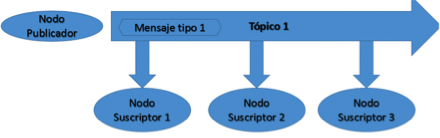
\includegraphics[width=0.8\textwidth]{figures/publicadorsubscriptor.png}
		\caption{Estructura del sistema de comunicación Publicador - Subscriptor}
		\label{fig.publicadorsubscriptor}
		\end{center}
\end{figure}

El sistema de comunicación síncrona, es el típico sistema cliente-servidor a través del cual un nodo ROS es el prestador del servicio que permanece en escucha continua y el resto de nodos le envían mensajes de solicitud. Cada servicio esta definido por el tipo de servicio que define la cantidad y tipo de datos que necesita el servicio tanto para recibir como petición, como para enviar como respuesta.

\begin{figure}[H]
  \begin{center}
    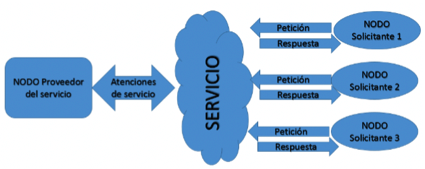
\includegraphics[width=0.8\textwidth]{figures/serviciosros.png}
		\caption{Estructura del sistema de comunicación por Servicios ROS}
		\label{fig.serviciosros}
		\end{center}
\end{figure}

Un elemento que es muy útil para este proyecto es que ROS nos proporciona total compatibilidad con Gazebo mediante un conjunto de paquetes llamados \textit{gazebo\_ros\_pkgs} \footnote{\url{http://wiki.ros.org/gazebo_ros_pkgs}}. En ROS, los paquetes son aquellos donde se incluye todo el código fuente, las librerías usadas y cualquier otro recurso necesario para que funcione el nodo.

\subsection{Robot Web Tools}
Comunidad nacida a partir de la de ROS, nos permite conectar aplicaciones web a elementos robóticos gracias a un protocolo llamado Rosbridge. Este protocolo es una especificación de JSON para interactuar con ROS y una capa de transporte para que los clientes se comuniquen mediante WebSockets. Por otro lado, han creado una serie de bibliotecas livianas y fáciles de utilizar de JavaScript que proporcionan una  abstracción de la funcionalidad principal de ROS. Estas bibliotecas son roslibjs, ros2djs y ros3djs, sin embargo en este trabajo solo se utilizara roslibjs.

La biblioteca roslibjs es la encarga de ofrecernos las funcionalidades necesarias para conectarnos, enviar o recibir mensajes ya sea mediante publicación y subscripción, o servicios. La conexión se realiza a un servidor intermedio (servidor Rosbridge), el cual se encarga de gestionar las conexiones, los topic publicados o los servicios activos en cada momento, de modo que cuando te subscribas o realices la petición de un servicio, este servdor se encargue de encaminar la petición mediante WebSockets.

Dado que para este trabajo se va a utilizar JavaScript como lenguaje, se utilizara, en todas las partes relacionadas con ROS, las bibliotecas, servidores y protocolo indicado en esta sección.

\begin{figure}[H]
  \begin{center}
    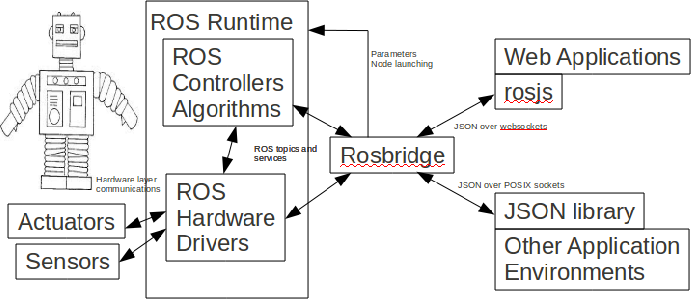
\includegraphics[width=0.8\textwidth]{figures/estructurarosbridge.png}
		\caption{Estructura de una aplicación con Rosbridge}
		\label{fig.estructurarosbridge}
		\end{center}
\end{figure}

\section{El entorno ICE}
Se trata de un Framework orientado a objetos que ayuda a crear aplicaciones distribuidas fácilmente. ICE se ocupa de todas las interacciones con las interfaces de programación de bajo nivel de red (inhibe al desarrollador de la tarea de apertura de puertos, conexiones de red o serialización de datos). El objetivo principal de ICE es facilitar su uso y el desarrollo de aplicaciones, de modo que en muy poco tiempo se pueda aprender a utilizarlo.

\begin{figure}[H]
  \begin{center}
    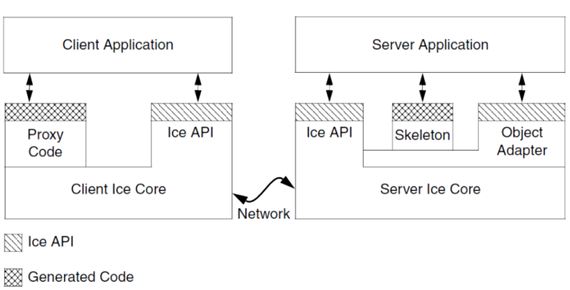
\includegraphics[width=0.8\textwidth]{figures/estructuraice.png}
		\caption{Estructura de Cliente - Servidor con Ice}
		\label{fig.estructurarice}
		\end{center}
\end{figure}

ICE tiene un lenguaje de especificación propio llamado Slice (Specification Language for ICE) que nos permite la abstracción fundamental para separar interfaces de objetos de sus implementaciones. Este lenguaje especifica las interfaces, operaciones y tipos de parámetros utilizados por nuestra aplicación. Cada una de las aplicaciones que queramos que interaccionen entre sí, deben compartir la misma descripción Slice. Esta descripción es independiente del lenguaje en el que está desarrollada nuestro cliente o servidor de modo que sea posible su utilización con clientes y servidores escritos en diferentes lenguajes de programación.

Para este trabajo se va a utilizar su versión para JavaScript, sin embargo el soporte para este lenguaje es relativamente reciente, por lo que muchas de las funcionalidades que ofrece para otros lenguajes de programación como C++ o Python, no están disponibles para JavaScript. Sobre todo este hecho es manifiesto en que no hay soporte para la creación de un servidor completo mediante JavaScript, por ello durante este trabajo se ha optado por utilizar ICE únicamente como cliente, con los ventajas e inconvenientes a los que se hará referencia en próximos capítulos.

\section{La plataforma JdeRobot}
JdeRobot \footnote{\url{https://jderobot.org/Main_Page}} es el framework de software libre para el desarrollo de robótica y visión artificial creado por el grupo de robótica de la Universidad Rey Juan Carlos y licenciado bajo GPL v3 \footnote{\url{http://www.gnu.org/licenses/gpl-3.0-standalone.html}}. Su desarrollo principalmente esta realizado mediante C, C++ y Python, incorporando desarrollo en JavaScript como el tratado en este trabajo.

JdeRobot esta basado en componentes que son interconectados mediante el uso de middlewares como ICE o ROS, facilitando el acceso a los dispositivos hardware. Estos componentes obtienen mediciones  de los sensores u ordenes del motor a través de llamadas a funciones locales. JdeRobot conecta esas llamadas a drivers conectados a sensores (para la recepción de las mediciones) o actuadores (para las ordenes), ya sean reales o simulados. Estas funciones locales forman la API de la capa de abstracción. La plataforma también ofrece una serie de herramientas para facilitar la teleoperación o el tratamiento de las mediciones de los sensores, y bibliotecas.
